
\documentclass[russian,12pt]{article}

\usepackage[utf8]{inputenc}
\usepackage[a4paper,left=20mm,right=20mm, top=20mm,bottom=20mm,bindingoffset=0cm]{geometry}
\usepackage{cmap}
\usepackage{indentfirst}
\usepackage[T2A]{fontenc}
\usepackage[russian]{babel}
\usepackage{amsfonts,amssymb,amsmath,amsthm}
\usepackage{hyperref}
\usepackage{graphicx}
\newtheorem{theorem}{Теорема}
\newtheorem*{theorem*}{Теорема А}
\newtheorem{theoremA}{Теорема A}
\newtheorem{lemma}{Лемма}
\newtheorem{suggestion}{Предложение}
\newtheorem{definition}{Определение}
\newtheorem{note}{Замечание}
\newcommand*{\defeq}{\stackrel{\text{def}}{=}}

\title{Как вода точит камень}
\author{Власов Алексей, Литвинов Марк\\
vlasoff.al03@gmail.com, mark.litvinov.2003@mail.ru\\
Научные руководители: Челноков Григорий Ривенович,\\Христофоров Михаил Игоревич}

\date{\today}



\begin{document}
\maketitle

Данная работа~--- исследование модели протекания воды из физики. В последнее время она представляет интерес для ученых, в ней сравнительно недавно были получены свежие результаты. В работе содержится доказательство \hyperref[main-theorem]{Теоремы A}, использующее остальные предложения, леммы и теоремы без доказательств.

Работа была проделана на \href{https://sochisirius.ru/obuchenie/nauka/smena880/4228}{майской проектной программе 2021 года в Сириусе}. Мотивировка предложенных результатов дана в \href{https://www.dropbox.com/sh/ayulkt9ysl91819/AAAuiWwPJy20kZui9A_rEXnCa?dl=0&preview=discrete-20.05.pdf}{проекте "Как вода  точит камень"}.

\bigskip

\section*{Вводные определения и постановка задачи}

Мы будем работать на действительной плоскости и отождествлять точки с комплексными числами естественным образом.

\begin{definition} \label{tau}
$\tau \in \mathbb{C}$ - комплексный корень $3$-й степени из 1, равный $-\frac{1}{2} + \frac{\sqrt{3}}{2}i$.
\end{definition}

\begin{definition}
$n$-замощением назовем любое замощение плоскости равными правильными шестиугольниками без просветов и наложений со стороной $\frac{1}{n}$ ориентированных так, что одна из сторон шестиугольников параллельна вектору $i$. 
\end{definition}
\begin{definition}
$M_n$ назовем множество шестиугольников из $n$-замощения, попавших внутрь треугольника с вершинами в точках $A = 1$, $B = \tau$, $C = \tau^2$.
\end{definition}
\begin{definition}
Назовем раскраской $M_n$ любую покраску шестиугольников из $M_n$ в 2 цвета: желтый и синий.\footnote{всего различных раскрасок $2^ {\#M_n}$, где $\#M_n$ - количество шестиугольников в $M_n$}.
\end{definition}
\begin{definition}
Будем говорить, что \emph{вода протекает между двумя ломаными}, проходящими по периметру границы $M_n$, если существует последовательность синих шестиугольников $a_1, a_2, \dots, a_k \in M_n$ такая, что $a_i$ имеет общую сторону с $a_{i+1}$, для всех $i=1,2 \dots, k-1$, и что одна из сторон $a_1$ является частью первой ломаной, одна из сторон $a_k$ - частью второй ломаной.
\end{definition}
\begin{definition}
Вероятность протекания для двух данных ломаных - доля всевозможных раскрасок шестиугольников из $M_n$ таких, что между этими ломаными протекает вода.
\end{definition}

\begin{definition}
$u_n(Z)$ - точка, являющаяся серединой стороны шестиугольника $M_n$, ближайшая для данной точки Z комплексной плоскости. Если таких точек несколько, выбирается любая.
\end{definition}
\begin{note}
Стоит отметить, что на самом деле $u$ - функция двух переменных: $\mathbb{C} \times \mathbb{N} \rightarrow \mathbb{C}$. Ее аргумент - пара из точки комплексной плоскости, номера выбранного замощения и его расположения, а множество значений - середины отрезков $n$-замощения. 
\end{note}

\begin{definition}\label{lomanaya}
Пусть $X, Y \in \mathbb{C}$,  $u_n(X)$ и $u_n(Y)$ лежат на границе $M_n$. Ломаной, соответствующей отрезку $XY$, назовем кратчайший участок границы $M_n$ от $u_n(X)$ до $u_n(Y)$. Если их несколько, выберем любой.
\end{definition}
\begin{note}
Далее это определение будет использовано только для отрезков $AB$ и $CD$.
\end{note}
\smallskip
\begin{theorem*}[С.Смирнов, 2001]\label{main-theorem}
Пусть $D$ - некоторая фиксированная точка на стороне $AC$ в треугольнике $ABC$. Тогда предел при $n \to \infty$, к которому стремится вероятность протекания между ломаными, соответствующим отрезкам $AB$ и $CD$, равен величине $\frac{CD}{AB}$.
\end{theorem*}
\smallskip

\begin{figure}[!ht]
\begin{center}
  \vspace{-0.3cm}
  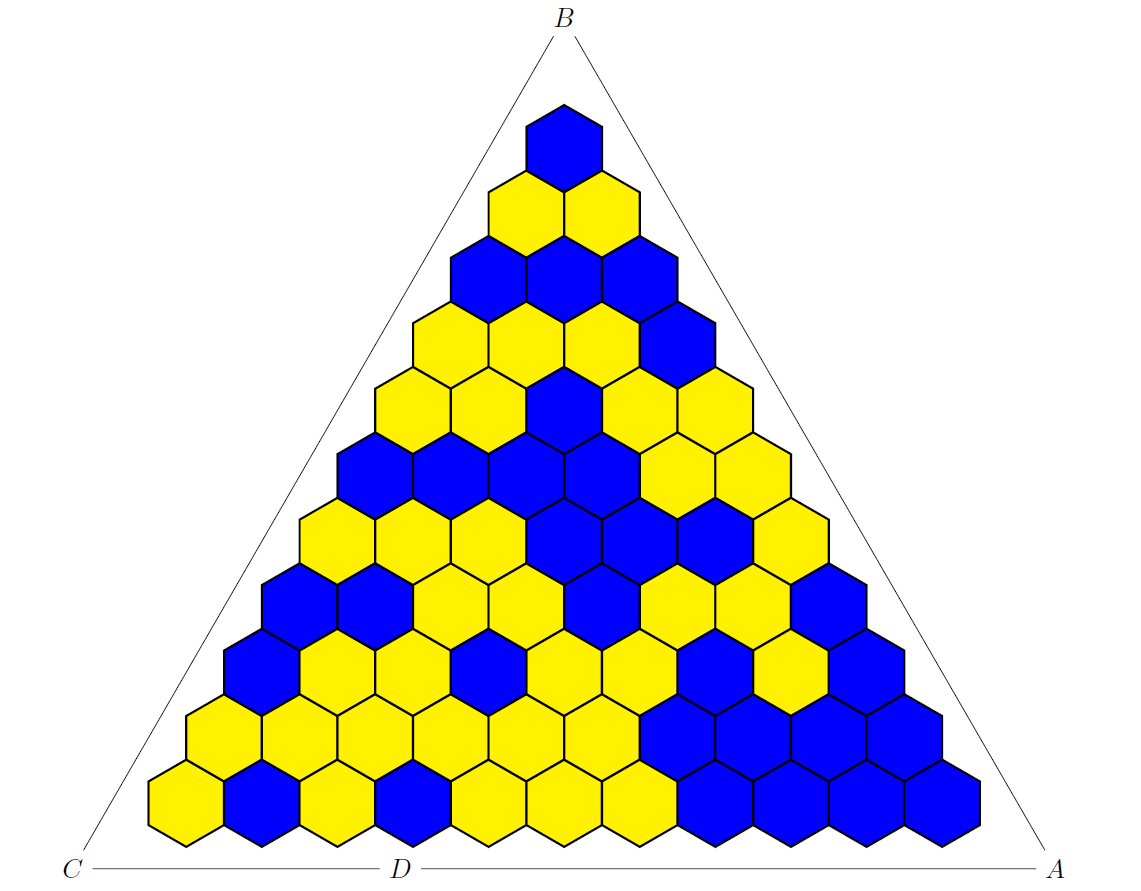
\includegraphics[width=0.3\textwidth]{triangle-v4.png}
  \vspace{-0.9cm}
\end{center}
  \caption{Модель протекания воды}
  \label{fig-simulation}
  \vspace{-1cm}
\end{figure}
\bigskip
\section*{Пути из красных отрезков}

Для решения задачи нам будет удобно перейти от раскрасок к ломаным, обладающим некоторыми свойствами. 

Целью этого перехода является формулировка и доказательство предложения \ref{2.14}. А сейчас опишем, как именно мы осуществим переход.
\begin{definition}
Для фиксированных $A = 1,$ $B = \tau,$ $C = \tau^2,$ $D \in \mathbb{C}$ и $n$-замощения будем называть \textbf{конфигурацией с особенностями $\boldsymbol{u_n(A)}$, $\boldsymbol{u_n(B)}$, $\boldsymbol{u_n(C)}$, $\boldsymbol{u_n(D)}$} множество ребер такого графа, что его вершинами являются вершины шестиугольников $M_n$ и все середины их ребер,
а его ребра соединяют вершину шестиугольника с серединой ребра, исходящего из нее. При этом ребра, составляющие конфигурацию, устроены так, что степень вершин  $u_n(A)$, $u_n(B)$, $u_n(C)$, $u_n(D)$ равна 1, а всех остальных - либо 0, либо 2.
\end{definition}
\begin{note}
Каждая конфигурация с особенностями представляет собой объединение двух простых путей, соединяющих $4$ особенные точки, и некоторого количества простых циклов.
\end{note}

Несложно понять, что все конфигурации разбиваются на три непересекающихся множества: в первом есть пути $u_n(A)u_n(B)$ и $u_n(C)u_n(D)$; во втором пути $u_n(A)u_n(C)$ и $u_n(B)u_n(D)$; в третьем $u_n(A)u_n(D)$ и $u_n(B)u_n(C)$. Тогда осмысленным становится следующее определение.

\begin{definition}
Зафиксируем $n$, $n$-замощение и точки $A$, $B$, $C$, $D$ на комплексной плоскости. Для них рассмотрим все конфигурации с особенностями в $u_n(A)$, $u_n(B)$, $u_n(C)$, $u_n(D)$. Обозначим за $P(u_n(D)\leftrightarrow u_n(A))$ долю конфигураций с особенностями $u_n(A)$, $u_n(B)$, $u_n(C)$, $u_n(D)$, где точки $u_n(A)$ и $u_n(D)$ - концы одной ломаной. При этом доопределим $P(u_n(A)\leftrightarrow u_n(A)) = 1$.
\end{definition}

Данные понятия формулировались для следующего предложения:



\begin{suggestion}\label{2.14}
Пусть дан $M_n$ и точки $u_n(A), u_n(B), u_n(C), u_n(D)$ на его границе. Тогда при фиксированном $n$: $P(u_n(D)\leftrightarrow{}u_n(A))$ равняется вероятности протекания воды по шестиугольникам между ломаными $u_n(A)u_n(B)$ и $u_n(C)u_n(D)$, соответствующим отрезкам $AB$ и $CD$ при данном $n$.
\end{suggestion}

\begin{proof}
Для доказательства утверждения покажем равносильность наличия протекания между указанными ломанными и наличия красного пути между вершинами $u_n(A)$ и $u_n(D)$. Сразу заметим: способ покраски ломаной в красный цвет на границе выбран так, что можно считать внешний граничный слой клеток окрашенным в синий цвет на границе с ломаными $u_n(A)u_n(B)$ и $u_n(C)u_n(D)$, а на границе с ломаными $u_n(B)u_n(C)$ и $u_n(D)u_n(A)$. При этом клетки вне $M$, одними из середин ребер которых являются $u_n(A), u_n(B), u_n(C), u_n(D)$ окрашены в оба цвета одновременно.
\newline
$\Rightarrow{}$ Пусть имеется протекание между ломаными $u_n(A)u_n(B)$ и $u_n(D)u_n(C)$. Заметим, что данное протекание делит шестиугольники на две части. Тогда $u_n(A)$ не может быть соединена ни с $u_n(B)$, ни с $u_n(C)$, так как они лежат по разные стороны от протекания, а через него ребра не проходят. Значит $u_n(A)$ соединена с $u_n(D)$.
\newline
$\Leftarrow{}$ Пусть имеется красный путь из $u_n(A)$ в $u_n(D)$. Тогда ближайший слой клеток по разные стороны от этого пути - цепочки из одноцветных шестиугольников, одна из которых будет синей, а другая желтой. Рассмотрим синюю: некоторые ее шестиугольники может быть окажутся за границей $M$. Это возможно только на границах $u_n(A)u_n(B)$ и $u_n(C)u_n(D)$. Отбросим их, тогда получится, что у нас есть синий путь от ломаной $u_n(A)u_n(B)$ до $u_n(C)u_n(D)$, что и требовалось.

\end{proof}

\section*{Наблюдаемая функция}

\begin{definition}
Для $n$-замощения введем функцию на множестве  середин всех сторон шестиугольников из $M_n$, включая $u_n(A),u_n(B),u_n(C)$ ($\tau$ определено в \ref{tau}):
$$
f_n(u_n(D)) \defeq P(u_n(D)\leftrightarrow u_n(A))
+\tau\,P(u_n(D)\leftrightarrow u_n(B)) +\tau^2\,P(u_n(D)\leftrightarrow u_n(C))
$$

\end{definition}
%В следующих двух предложениях мы сформулируем хорошие свойства этой функции, из которых  последует сходимость последовательности таких функций к аналитической.

\begin{suggestion} \label{3.1a}
Пусть $z$ --- общая вершина трех шестиугольников из $M_n$.
Пусть $p,q,r$ --- середины их общих сторон, перечисленные в порядке против часовой стрелки. Тогда для функции $f_n$ выполняется тождество треугольника:
\begin{equation}\label{eq-l-discrete-analiticity}
    (p-z)f_n(p)+(q-z)f_n(q)+(r-z)f_n(r)=0.
\end{equation}
\end{suggestion}


Следующее предложение является более удобным следствием предыдущего.

\begin{suggestion} \label{3.1b}
Рассмотрим цепочку из $k$ шестиугольников из $M_n$, в которой соседние шестиугольники имеют общую сторону, и последний имеет общую сторону с первым. Обозначим через $w_1,\dots, w_{k}$ центры этих шестиугольников и положим $w_{k+1}:=w_1$. Тогда если $f(z)$ --- любая функция, удовлетворяющая тождеству треугольника и определенная на множестве середин сторон шестиугольников $n$-замощения из $M_n$, то
\begin{equation} \label{analit}
\sum\limits_{j=1}^{k} f\left(\frac{w_{j+1}+w_{j}}{2}\right) (w_{j+1}-w_{j})=0.
\end{equation}
\end{suggestion}


\begin{proof}[Доказательство предложения \ref{3.1b}] 
Соединим $w_j$ с $w_{j+1}$, получим цикл $\psi$. Рассмотрим все узлы шестиугольной решетки, которые расположены внутри цикла $\psi$. Напишем для каждого из этих узлов тождество треугольника. Сложим все полученные равенства. Тогда для любой середины $Z$ отрезка $AB$ находящейся строго внутри этого цикла, $f(z)$ будет посчитано с коэффициентами $z-a$ и $z-b$, то есть с коэффициентом $2z-a-b=0$. Тогда в сумме останутся только вершины вида $\frac{w_{j+1} + w_j}{2}$ с коэффициентами $\frac{w_{j+1} + w_j}{2} - w$, где $w$ - тот узел, в котором посчитана эта середина. Домножим полученное равенство на $2\sqrt{3}i$. Тогда вектор $\frac{w_{j+1} + w_j}{2} - w$ перейдет в вектор $w_{j+1} - w_j$. Мы получили равенство \ref{analit}.
\end{proof}

\begin{note}
Это дискретная переформулировка стандартного определения аналитичности.
\end{note}

\section*{Ключевые утверждения}

\begin{theorem} \label{3.3}
Существует функция $F(Z)$, заданная на всем треугольнике $ABC$, включая границу, и
принимающая комплексные значения, такая что $$\displaystyle \lim_{n\to\infty}\max_{Z\in{}ABC}{{|F(Z) - f_n(u_n(Z))|}} = 0.$$
\end{theorem}

Эта теорема не будет доказана в данной статье, больше о ней можно прочитать, например, \href{https://ru.wikipedia.org/wiki/%D0%A2%D0%B5%D0%BE%D1%80%D0%B5%D0%BC%D0%B0_%D0%90%D1%81%D0%BA%D0%BE%D0%BB%D0%B8_%E2%80%94_%D0%90%D1%80%D1%86%D0%B5%D0%BB%D0%B0}{здесь}.

\begin{suggestion} \label{3.4a}
Функция $F(Z)$ из теоремы \ref{3.3} непрерывна:
\begin{equation}
\displaystyle \lim_{n\to\infty}\max_{Z\in{}ABC}{{|F(Z) - F(u_n(Z))|}} = 0.
\end{equation}
\end{suggestion}



\begin{proof}
Для начала докажем следующий факт: $$\displaystyle \lim_{n\to\infty}\max_{Z\in{}ABC}{{|F(u_n(Z)) - f_n(u_n(Z))|}} = 0$$
Зафиксируем $\varepsilon_0 > 0$. Тогда по определению функции $F(Z) : \exists n_0 \in \mathbb{N}: \forall n > n_0 : \forall Z \in ABC: |F(Z) - f_n(u_n(Z))| < \varepsilon_0$. Поскольку этот факт верен для любой точки $Z$ и ближайшей к ней середине $n$-замощения $u_n(Z)$, то в частности можно выбрать в роли $Z$ саму точку $u_n(Z)$.
\\ \\
Теперь докажем теорему.
Зафиксируем $\varepsilon_0 > 0$. Тогда по определению функции $F(Z)$ и вышедоказанному утверждению $\exists n_0 \in \mathbb{N}: \forall n > n_0 : \forall Z \in ABC: |F(Z) - F(u_n(Z))| \leq |F(Z) - f_n(u_n(Z))| + |F(u_n(Z)) - f_n(u_n(Z))| \leq \frac{\varepsilon_0}{2} + \frac{\varepsilon_0}{2} = \varepsilon_0$.
\end{proof}

\begin{suggestion} \label{3.4b}
Для любого правильного треугольника $PQR$, гомотетичного $ABC$ и лежащего строго внутри $ABC$, и функции $F(Z)$ из теоремы \ref{3.3} выполнено:
\begin{equation}
\lim_{n\to\infty} \sum\limits_{j=1}^{l_n} F\left(\frac{w_{j+1,n}+w_{j,n}}{2}\right) (w_{j+1,n}-w_{j,n})=0,
\end{equation}
где $w_{1,n},w_{2,n},\dots,w_{l_n,n}$ --- центры шестиугольников $n$-го замощения, пересекающих контур треугольника $PQR$, занумерованных в порядке обхода этого контура против часовой стрелки.
\end{suggestion}



\begin{proof}[Доказательство теоремы \ref{3.4b}] 
Докажем, что:
$$\forall \varepsilon > 0 \space \exists \space n_0 : \forall n > n_0 \left|\sum_{j=1}^{l_n} F \left( \frac{w_{j+1} + w_j}{2} \right) ({w_{j+1} - w_j}) \right| < \varepsilon$$
По определению функции $F(z)$:
$$\forall \varepsilon > 0 \space \exists \space n_0 : \forall n > n_0 \left| F(Z) - f_n(u_n(Z)) \right| < \varepsilon$$
Мы уже знаем, что по предложению \ref{3.1b}:
$$\sum_{j=1}^{l_n} f_n \left( \frac{w_{j+1} + w_j}{2} \right) ({w_{j+1} - w_j}) = 0$$
Вычтем это из подмодульного выражения:
$$\left|\sum_{j=1}^{l_n} \left( F \left( \frac{w_{j+1} + w_j}{2} \right) - f_n \left( \frac{w_{j+1} + w_j}{2} \right) \right) ({w_{j+1} - w_j}) \right|$$
По неравенству треугольника мы можем оценить это сверху, как:
$$
\sum_{j=1}^{l_n} \left| F \left( \frac{w_{j+1} + w_j}{2} \right) - f_n \left( \frac{w_{j+1} + w_j}{2} \right) \right| \left| ({w_{j+1} - w_j}) \right|    
$$
$|w_{j+1} - w_j| = \frac{\sqrt{3}}{n}$, поскольку сторона шестиугольников $\frac{1}{n}$. По выбору $n$ мы получаем, что: 
$$\left| F \left( \frac{w_{j+1} + w_j}{2} \right) - f_n \left( \frac{w_{j+1} + w_j}{2} \right) \right| < \varepsilon$$
Значит мы можем оценить нашу сумму сверху, как $l_n\varepsilon\frac{\sqrt{3}}{n}$.
Заметим, что для любых двух соседних шестиугольников участок границы $PQR$ находящийся внутри них $\geq \frac{1}{n}$. Пусть длина границы $PQR$ - $a$. Тогда $\frac{l_n}{2n} \leq a$, иначе получилось бы, что граница $PQR$ внутри шестиугольников больше длины границы $PQR$. А значит $\frac{l_n}{n} \leq 2a$, следовательно $l_n\varepsilon\frac{\sqrt{3}}{n} \leq 2\sqrt{3}\varepsilon a$, что бывает сколь угодно малым при правильном выборе $\varepsilon$.  
\end{proof}

\begin{definition}
Обозначим через $[z;w]$ выпуклую оболочку векторов $z$ и $w$, где  $z,w\in\mathbb{C}$, иначе говоря $[z;w] \defeq \{z + \lambda(w - z) \space | \space \forall \space \lambda \in [0, 1] \}$.
\end{definition}

\begin{suggestion} \label{3.4c}
 Для любой точки $D$ на границе треугольника $ABC$ функция $F(Z)$ из теоремы \ref{3.3} удовлетворяет условию: 
 $$
 F(D) \in 
 \begin{cases}
 [1; \tau{}^2] &\text{при D $\in$ [A, C],} \\
 [\tau{}^2; \tau{}] &\text{при D $\in$ [C, B],} \\
 [\tau{}; 1] &\text{при D $\in$ [B, A].} \\
 \end{cases}
 $$
 
\end{suggestion}



\begin{proof}
Пусть точка $D$ лежит на отрезке $[A, C]$. Тогда из определения функции $F(Z)$ имеем:
$$F(D) = \displaystyle \lim_{n\to\infty} {f_n(D_n)}$$
Поскольку $D$ лежит на отрезке $AC$, то ближайшая к ней середина $u_n(D)$ лежит на границе многоугольника $M_n$. Отсюда $P(u_n(B) \leftrightarrow u_n(D)) = 0$, так как если она не равна 0, то существует расположение ломаных, соединяющих $u_n(A)$ и $u_n(C)$, $u_n(B)$ и $u_n(D)$, но в таком случае они пересекаются $ \Rightarrow$ противоречие.
\\
Тогда: $\forall n \in \mathbb{N}: P(u_n(B) \leftrightarrow u_n(D) = 0 \Rightarrow f_n(u_n(Z))=P(u_n(D) \leftrightarrow u_n(A)) + {\tau{}^2}P(u_n(D) \leftrightarrow u_n(C))$
\\
Иными словами $f_n(u_n(Z))$ представляется в виде выпуклой комбинации векторов $1$ и $\tau{}^2$, и значит при всех $n$ лежит на отрезке $AC$. Тогда и предел, поскольку он существует, лежит на этом отрезке. Тогда $F(D) \in [AC]$. Что и требовалось. Остальные случаи разбираются аналогично.
\end{proof}

\begin{theorem} \label{3.5} 
Существует не более одной функции $F(Z)$, заданной на всем треугольнике $ABC$, включая границу, принимающей комплексные значения и удовлетворяющей свойствам
из предыдущих трех предложений.
\end{theorem}

Это утверждение является классическим результатом комплексного анализа и не будет доказано в этой статье.

\begin{lemma}\label{f=z}

Тождественная функция $F(Z) = Z$ удовлетворяет предложениям: \ref{3.4a}, \ref{3.4b}, \ref{3.4c}.

\end{lemma}



\begin{proof}
По порядку докажем все три утверждения:

1. Тождественная функция непрерывна.

2. Покажем аналитичность:
\begin{multline*}
    \sum\limits_{j=1}^{l_n} F\left(\frac{w_{j+1,n}+w_{j,n}}{2}\right) (w_{j+1,n}-w_{j,n})= \sum\limits_{j=1}^{l_n} \frac{1}{2}(w_{j+1,n}+w_{j,n}) (w_{j+1,n}-w_{j,n})= \\ =  \frac{1}{2}\sum\limits_{j=1}^{l_n} (w_{j+1,n}^2-w_{j,n}^2)  = 0
\end{multline*}

Выражение обращается в нуль, поскольку каждое слагаемое в виде квадрата встречается с плюсом и минусом.

3. Граничное условие для тождественной функции верно в силу выбора расположения точек $A, B, C$. 
\end{proof}

\subsection*{Доказательство Теоремы А}
Мы ищем предел вероятности протекания воды между ломаными, соответствующими сторонам $AB$ и $CD$ при $n \to \infty$. Иными словами мы ищем предел некоторой последовательности. По предложению \ref{2.14} члены этой последовательности совпадают с членами последовательности $\{P(u_n(D) \leftrightarrow u_n(A))\}$. Тогда нам достаточно найти  $\lim_{n \to \infty}P(u_n(D) \leftrightarrow u_n(A))$

Из леммы \ref{f=z} и теоремы \ref{3.5} мы получаем, что определенная в теореме \ref{3.3} функция $F(z)$ - тождественная функция. В частности, $F(D) = D$.

Тогда с одной стороны:
$$D = F(D) = \lim_{n \to \infty} f_n(u_n(D)) = \lim_{n \to \infty} \left( P(u_n(D) \leftrightarrow u_n(A)) + \tau^2P(u_n(D) \leftrightarrow u_n(C)) \right)$$
Но, с другой стороны, точка $D$ представима единственным образом в виде выпуклой комбинации $1$ и $\tau^2$: 
$$D = 1*\frac{DC}{AC} + \tau^2*\frac{AD}{AC} \Rightarrow \lim_{n \to \infty}  P(u_n(D) \leftrightarrow u_n(A)) = \frac{DC}{AC}$$
Это в точности то, что мы хотели доказать!

\end{document} 